% !TeX root = ../main.tex

% Tighten vertical spacing for this chapter only
\titlespacing*{\section}{0pt}{2ex plus .5ex minus .2ex}{0.3ex}
\titlespacing*{\subsection}{0pt}{1.5ex plus .3ex minus .2ex}{0.2ex}
\titlespacing*{\subsubsection}{0pt}{1.2ex plus .3ex minus .2ex}{0.2ex}
\setlength{\parskip}{4pt}

\chapter[Dataset and Experiment Setting]{Dataset and \\ Experiment Setting}
\label{chap:setup}

This chapter describes the data and the experimental protocol used throughout the thesis. Section~\ref{sec:dataset} introduces the NTUH Parkinson's Disease outpatient clinic dataset, its two temporal cohorts, the medication-status sub-groups, and the joint-major feature layout. Section~\ref{sec:roadmap} then lays out the roadmap of the five experiments, and Section~\ref{sec:exp_setting} details the evaluation protocols, fold-wise preprocessing, evaluation metrics, and model hyperparameter settings.

\section{NTUH Parkinson's Disease Outpatient Clinic Dataset}
\label{sec:dataset}

This study uses a clinical dataset collected at the National Taiwan University Hospital (NTUH) Parkinson's Disease outpatient clinic in collaboration with Dr.~Lin Jing-Xian (林靜嫻). All recordings were captured as 2D videos using the camera of an ordinary smartphone or tablet, so that the resulting cohort is directly representative of the everyday-device scenario targeted by this thesis.

The data come in two temporal cohorts. The \emph{2020 cohort} consists of recordings of variable length collected starting in 2020. The \emph{2025 cohort} consists of recordings standardized to a fixed length of 30 seconds, collected starting in 2025. Together with the medication status of each subject at recording time, these two cohorts form four sub-groups: 2020/on-medication, 2020/off-medication, 2025/on-medication, and 2025/off-medication.

Table~\ref{tab:dataset_overview} contrasts the high-level properties of the two cohorts.

\begin{table}[H]
    \centering
    \caption{High-level comparison of the 2020 and 2025 cohorts}
    \label{tab:dataset_overview}
    \small
    \setlength{\tabcolsep}{8pt}
    \begin{tabularx}{\linewidth}{>{\raggedright\arraybackslash}p{0.40\linewidth} >{\raggedright\arraybackslash}X >{\raggedright\arraybackslash}X}
        \hline
        Aspect & 2020 cohort & 2025 cohort \\
        \hline
        Video duration                          & Variable                & Fixed 30~s \\
        Healthy:PD ratio under off-medication   & 134:57 ($\sim$7:3)      & 90:28 ($\sim$3:1) \\
        Number of on-medication subjects        & 79                      & 103 \\
        Number of off-medication subjects       & 191                     & 118 \\
        \hline
    \end{tabularx}
\end{table}

The detailed stage distribution of the two cohorts is shown in Table~\ref{tab:dataset_distribution}.

\begin{table}[H]
    \centering
    \caption{Sample distribution by MDS-UPDRS stage and medication status for the two cohorts}
    \label{tab:dataset_distribution}
    \small
    \setlength{\tabcolsep}{5pt}
    \begin{tabularx}{\linewidth}{l l c c c c c c}
        \hline
        Cohort & Medication & Stage~0 & Stage~1 & Stage~2 & Stage~3 & Stage~4 & Total \\
        \hline
        \multirow{2}{*}{2020} & On  & 0   & 19 & 32 & 24 & 4 & 79  \\
                                & Off & 134 & 13 & 27 & 16 & 1 & 191 \\
        \hline
        \multirow{2}{*}{2025} & On  & 0   & 39 & 34 & 20 & 9 & 102 \\
                                & Off & 90  & 15 & 8  & 4  & 1 & 118 \\
        \hline
    \end{tabularx}
\end{table}

Throughout this thesis, stage~0 is treated as the \emph{healthy} class and stages~1--4 are merged into the \emph{PD} class. To avoid confounding the underlying motor severity with the effect of levodopa therapy, all principal experiments restrict the analysis to off-medication recordings.

\subsection{Ethical Approval and Informed Consent}
\label{sec:ethics}

The clinical recordings were collected at the NTUH Parkinson's Disease outpatient clinic under the supervision of Dr.~Lin Jing-Xian. All participants provided informed consent for the use of their de-identified hand-rotation videos for research purposes prior to recording. The data shared with the present author for analysis contain no personally identifiable information.

\subsection{Subject Composition}
\label{sec:subject_overlap}

Both cohorts consist of recordings from independent subjects: the 191 off-medication recordings in the 2020 cohort and the 118 off-medication recordings in the 2025 cohort each originate from a distinct individual, so leave-one-out at the recording level is equivalent to leave-one-subject-out in both cases. The two cohorts share no overlapping subjects; the 2020-to-2025 cross-cohort transfer protocol of Section~\ref{sec:cross_cohort} therefore evaluates generalisation to a strictly disjoint set of subjects recorded under a different protocol.

\subsection{Feature Dimensionality}
\label{sec:feature_dim}

This subsection summarises how the 1,764-dimensional per-patient feature vector used throughout Chapters~\ref{chap:methods} and~\ref{chap:results} is assembled from the raw MediaPipe joint trajectories, so that the dimension counts referenced elsewhere in the thesis can be traced back to their source.

Each recording yields, per hand, 21 MediaPipe joints tracked along 3 spatial axes ($x$, $y$, $z$). For every single joint-axis trajectory, two autocorrelation-based descriptors (frequency, clarity) and four amplitude representations (cycle-by-cycle, rolling peak-to-peak, rolling RMS, Hilbert envelope)---each summarised by three statistics (mean, standard deviation, median)---are computed, as detailed in Section~\ref{sec:fe}. This gives $2 + 4 \times 3 = 14$ descriptors per axis. Table~\ref{tab:feature_dim_axis} lists these 14 descriptors explicitly.

\begin{table}[H]
    \centering
    \caption{Composition of the 14 descriptors computed per joint-axis trajectory}
    \label{tab:feature_dim_axis}
    \small
    \setlength{\tabcolsep}{8pt}
    \begin{tabularx}{\linewidth}{>{\raggedright\arraybackslash}p{0.28\linewidth} >{\raggedright\arraybackslash}X c}
        \toprule
        Descriptor family & Statistics & Dimensions \\
        \midrule
        Frequency          & --- (single scalar)             & 1 \\
        Clarity             & --- (single scalar)             & 1 \\
        Cycle-by-cycle amplitude    & Mean, Std, Median      & 3 \\
        Rolling peak-to-peak amplitude & Mean, Std, Median   & 3 \\
        Rolling RMS amplitude       & Mean, Std, Median      & 3 \\
        Hilbert envelope amplitude  & Mean, Std, Median      & 3 \\
        \midrule
        \textbf{Total per axis} & & \textbf{14} \\
        \bottomrule
    \end{tabularx}
\end{table}

Since each of the 3 spatial axes ($x$, $y$, $z$) independently contributes 14 such descriptors, a single joint yields $14 \times 3 = 42$ descriptors. With 42 joints per patient (21 joints $\times$ 2 hands), the total per-patient feature dimensionality is $42 \times 42 = 1{,}764$. Table~\ref{tab:feature_dim_overall} traces this hierarchical build-up from axis to joint to patient level.

\begin{table}[H]
    \centering
    \caption{Hierarchical composition of the 1,764-dimensional per-patient feature vector}
    \label{tab:feature_dim_overall}
    \small
    \setlength{\tabcolsep}{8pt}
    \begin{tabularx}{\linewidth}{>{\raggedright\arraybackslash}p{0.30\linewidth} >{\raggedright\arraybackslash}X c}
        \toprule
        Level & Composition & Dimensions \\
        \midrule
        Per axis            & 2 autocorrelation + 4 amplitude $\times$ 3 statistics  & $2 + 4\times3 = 14$ \\
        Per joint            & 3 axes ($x,y,z$) $\times$ 14 descriptors               & $14 \times 3 = 42$ \\
        Per patient          & 42 joints (21 joints $\times$ 2 hands) $\times$ 42 descriptors & $42 \times 42 = 1{,}764$ \\
        \bottomrule
    \end{tabularx}
\end{table}

This joint-major, 42-descriptors-per-joint structure is not merely bookkeeping: it is what allows the 1,764-dimensional vector to be reshaped into a 42-node joint graph, with 42 node-level descriptors per joint, for the graph-aggregated correlation features of Section~\ref{sec:joint_corr_corr} and the feature-based AGCN-style model of Section~\ref{sec:joint_corr_agcn}.

\section{Experimental Roadmap}
\label{sec:roadmap}

Five experiments are conducted in this thesis, each motivated by a specific research question concerning feature representation, feature dimensionality, lateralization effects, inter-joint correlation, and graph-based learning for PD-versus-healthy binary classification on the NTUH cohorts.

\textbf{Experiment~1} establishes a baseline by performing binary classification using two feature sets: thumb-tip features and full bilateral hand-joint features. Three classifiers are evaluated---Logistic Regression, Random Forest, and XGBoost---to assess the discriminative capacity of these features without any feature selection.

\textbf{Experiment~2} addresses the high feature dimensionality arising from bilateral joint representations. Feature selection is applied to the full bilateral hand-joint feature set using three methods---ANOVA F-test, L1-regularized Logistic Regression, and XGBoost feature importance---each followed by XGBoost binary classification.

\textbf{Experiment~3} repeats the pipeline of Experiment~2 separately on left-hand-only and right-hand-only feature subsets. By comparing the classification performance of each hand independently, this experiment aims to expose asymmetric motor decline and investigate the influence of motor reserve on PD discrimination.

\textbf{Experiment~4} extends the bilateral feature set with the 203-dimensional graph-aggregated joint-correlation descriptor described in Section~\ref{sec:joint_corr_corr}. This descriptor encodes inter-joint feature-profile similarity via a Ledoit-Wolf shrinkage correlation matrix, one step of GCN-style graph aggregation, node-level pooling, bilateral asymmetry statistics, and block-level intra/inter-hand coupling statistics. The resulting 1,967-dimensional extended feature vector is reduced by the same three feature-selection methods from Experiment~2, followed by XGBoost classification, to assess whether graph-structured inter-joint correlation improves discriminative performance.

\textbf{Experiment~5} evaluates a feature-based Adaptive Graph Convolutional Network style model (AGCN-style) on the full bilateral hand-crafted feature representation. Instead of constructing graph features analytically, the 1,764-dimensional feature vector is reshaped into a 42-node joint graph and the AGCN-style model learns both the graph topology and the classification boundary end-to-end through an adaptive adjacency mechanism, allowing the network to discover which joint interactions are most informative for PD classification while retaining the same kinematic descriptors used by the earlier experiments.

\section{Experimental Setting}
\label{sec:exp_setting}

\subsection{Within-Cohort Validation}
\label{sec:loocv}

Within a single cohort, a LOOCV protocol is employed to maximize the use of the limited clinical data. In each iteration, one subject is held out as the test sample and the remaining subjects constitute the training set. For Experiments~2--4, feature selection is re-executed on the training fold of every LOOCV iteration so that no information from the held-out subject can influence the selected feature subset. Fold-dependent preprocessing, including missing-value imputation, feature standardisation, and class-weight estimation, is likewise fit only on the training fold and then applied to the held-out subject. The out-of-fold predicted probability of each subject is stored, and the pooled probabilities are used to construct a single ROC curve per experimental configuration.

\subsection{Cross-Cohort Evaluation}
\label{sec:cross_cohort}

In addition to within-cohort LOOCV, a stricter cross-cohort transfer protocol is applied to assess generalization across recording conditions. The model is trained on the complete 2020 off-medication cohort and evaluated on the complete 2025 off-medication cohort. Feature selection is performed exclusively on the training cohort, and the resulting feature indices are applied without modification to the unseen test cohort. Accuracy, F1-score, and AUROC are reported on the test cohort.

\subsection{Fold-wise Preprocessing and Normalisation}
\label{sec:fold_preprocess}

All preprocessing operations that estimate distributional quantities are nested strictly inside the corresponding training split. Specifically:

\begin{itemize}
    \item \textbf{Imputation.} Missing numerical feature values are imputed with the per-feature median computed \emph{exclusively} from the training fold (LOOCV) or the source cohort (cross-cohort transfer). The same imputation values are then applied to the held-out sample or target cohort without re-estimation.
    \item \textbf{Standardisation.} When a standardised representation is required, \texttt{StandardScaler} is fit on the training data only and reused unchanged for the held-out fold or the 2025 test cohort. This applies to the baseline joint-feature classifiers, to the ANOVA and L1-regularised feature-selection paths, and to the feature-based AGCN-style model. XGBoost-based feature selection and final XGBoost classifiers do not require a separately standardised input scale.
    \item \textbf{Feature selection.} For Experiments~2--4, feature selection (ANOVA, L1-logistic, or XGBoost gain) is re-executed on the training fold of every LOOCV iteration and on the source cohort for cross-cohort transfer. The indices of the selected features are then applied to the held-out or target data without re-ranking.
    \item \textbf{Threshold selection.} The optimal classification threshold $\theta^{*}$ (Section~\ref{sec:metrics}) is estimated from training or out-of-fold predictions only; the 2025 cohort labels are never consulted during threshold selection.
\end{itemize}

This design ensures that neither the held-out sample in LOOCV nor the target cohort in cross-cohort transfer can influence the imputation values, the feature scale, the selected feature subset, or the decision threshold.

For the AGCN-style model, the fold-specific standardised 1,764-dimensional vector is reshaped into a 42-node graph, with 42 descriptors assigned to each bilateral hand-joint node. Class weights for the weighted cross-entropy loss are computed from the training data of the corresponding fold or source split.

\subsection{Evaluation Metrics}
\label{sec:metrics}

Model performance is evaluated using three complementary metrics: \emph{AUROC}, \emph{accuracy}, and \emph{F1-score}. AUROC is threshold-independent and serves as the primary metric for cross-model comparison. Accuracy and F1-score are threshold-dependent and require a fixed decision threshold; the optimal threshold is selected via the Youden index~\cite{youden1950index}, estimated only from training or validation predictions and held fixed for test evaluation.

The Youden index is defined as the maximum vertical distance from the ROC curve to the diagonal chance line:
\begin{equation}
    J(\theta) = \mathrm{TPR}(\theta) - \mathrm{FPR}(\theta),
    \label{eq:youden}
\end{equation}
where $\mathrm{TPR}(\theta)$ and $\mathrm{FPR}(\theta)$ denote the sensitivity and one-minus-specificity at classification threshold $\theta$, respectively. Geometrically, the diagonal represents a random classifier (AUROC $= 0.5$), and $J(\theta)$ measures how far the operating point departs from this baseline. The optimal threshold is
\begin{equation}
    \theta^{*} = \arg\max_{\theta}\; J(\theta),
    \label{eq:youden_opt}
\end{equation}
which simultaneously maximises sensitivity and specificity without imposing an \emph{a priori} cost asymmetry between false positives and false negatives.

\begin{figure}[H]
    \centering
    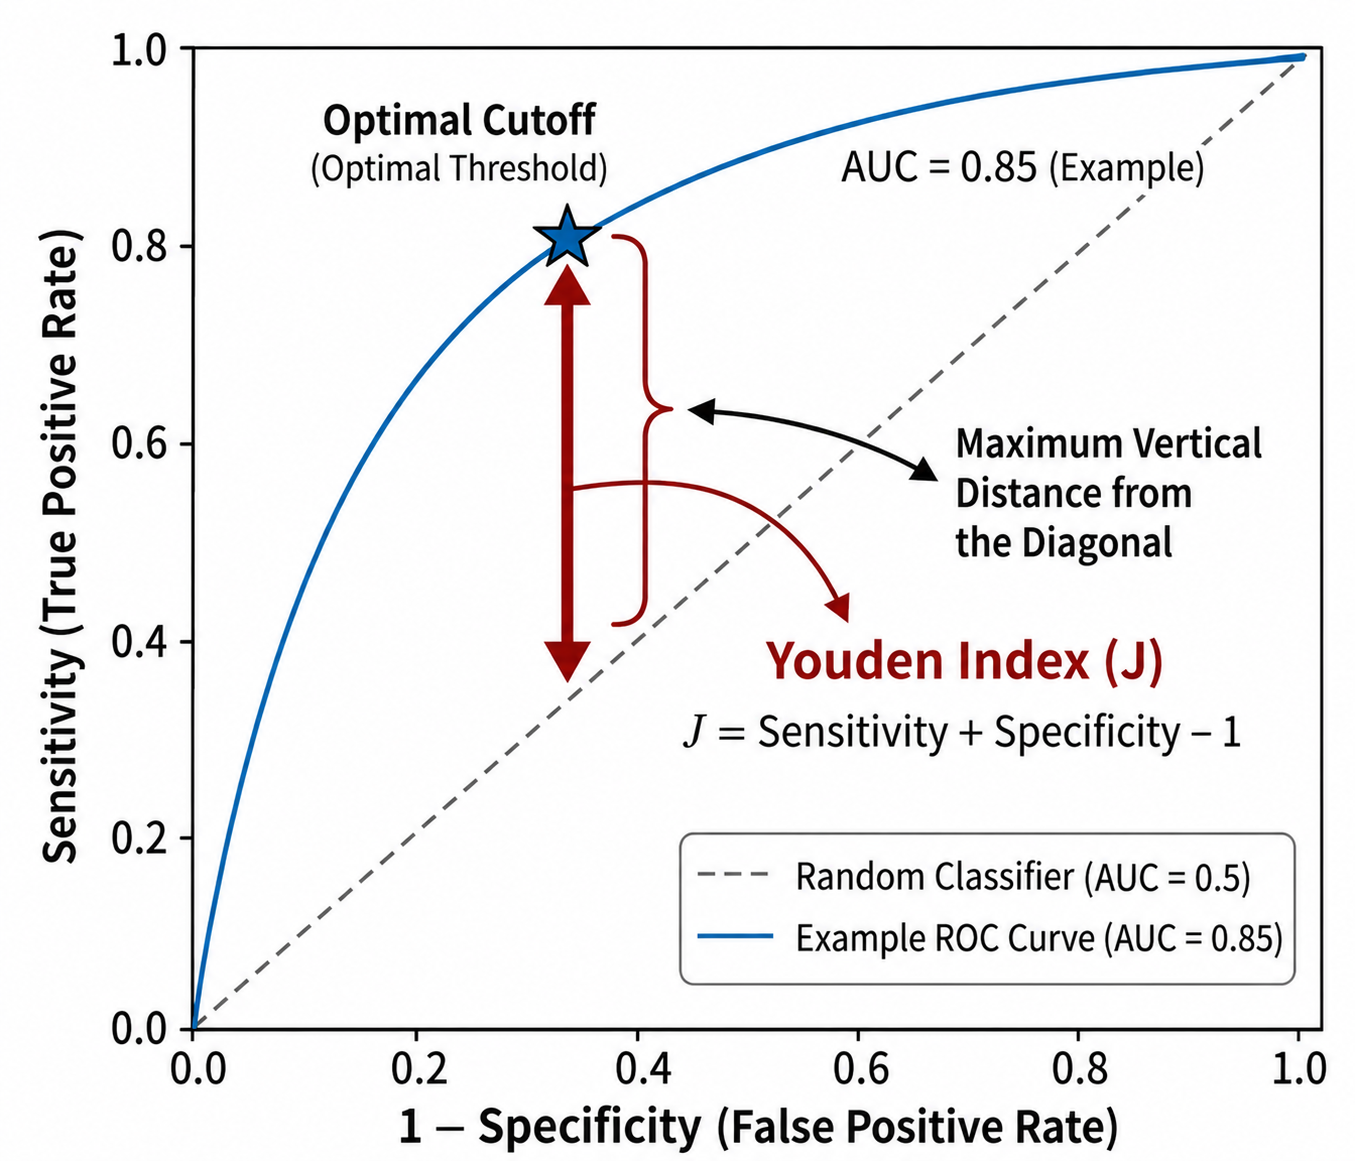
\includegraphics[width=0.55\linewidth]{figures/younden_index}
    \caption{Geometric interpretation of the Youden index on a representative ROC curve (AUC = 0.85). The index $J$ equals the maximum vertical distance from the curve to the chance diagonal; the optimal cutoff is the operating point achieving this maximum.}
    \label{fig:youden}
\end{figure}

Fig.~\ref{fig:youden} illustrates the geometric interpretation: the diagonal represents a random classifier (AUC $= 0.5$), and the starred point marks the threshold $\theta^{*}$ at which the vertical distance from the ROC curve to the diagonal is greatest.

This criterion is particularly suitable for clinical screening tasks. In medical datasets, class distributions are typically imbalanced and the cost of missing a true case (false negative) may differ substantially from the cost of a false alarm. The 0.5 default threshold---optimal only when classes are balanced and misclassification costs are equal---is therefore inappropriate. The Youden index selects the threshold that provides the best balance between sensitivity and specificity given the observed ROC curve, without requiring explicit specification of misclassification costs.

The practical estimation of $\theta^{*}$ differs between the two evaluation protocols and between the two model families, and these details are reported here for transparency.

For \emph{within-cohort LOOCV}, the out-of-fold predicted probability of every subject is accumulated across folds and $\theta^{*}$ is computed once from this pooled set of out-of-fold predictions. Because each predicted probability is generated by a model that has never seen the corresponding subject during training, this procedure is equivalent to using a validation-derived operating point in the conventional sense.

For \emph{cross-cohort transfer}, the operating point is estimated from the source cohort and reused unchanged on the 2025 test cohort. In the XGBoost feature-selection and graph-concat experiments, $\theta^{*}$ is computed from a source-cohort LOOCV pass on the 2020 training data; in the AGCN experiment, the threshold saved from the source-cohort LOOCV run is applied to the target cohort. The 2025 labels are used only for final metric computation. This avoids test-cohort threshold tuning for the reported accuracy and F1-score, while AUROC remains threshold-independent.

\subsection{Training-Termination Criteria}
\label{sec:termination}

Each model family adopts a stopping criterion appropriate to its optimization procedure.

\begin{itemize}
    \setlength{\itemsep}{0pt}
    \setlength{\parsep}{0pt}
    \setlength{\topsep}{0pt}
    \item \textbf{Logistic Regression} converges when the change in training loss between consecutive iterations falls below a predefined tolerance.
    \item \textbf{Random Forest} and \textbf{XGBoost} are trained for a fixed number of trees and nodes, respectively, as specified in Section~\ref{sec:exp_setting_hparams}.
    \item \textbf{AGCN-style model} is trained for at most 100 epochs and uses early stopping with a patience of 20 epochs without improvement in validation loss.
\end{itemize}

\subsection{Hyperparameters}
\label{sec:exp_setting_hparams}

The hyperparameters of the XGBoost and AGCN models used throughout the experiments are summarized in Tables~\ref{tab:xgboost_params} and~\ref{tab:agcn_params}.

\begin{table}[H]
    \centering
    \caption{Hyperparameter configuration for the XGBoost classifier}
    \label{tab:xgboost_params}
    \small
    \setlength{\tabcolsep}{12pt}
    \begin{tabularx}{\linewidth}{>{\raggedright\arraybackslash}X c}
        \hline
        Hyperparameter & Value \\
        \hline
        Number of estimators (\texttt{n\_estimators})       & 50 \\
        Maximum depth (\texttt{max\_depth})                  & 3 \\
        Learning rate (\texttt{learning\_rate})              & 0.1 \\
        Evaluation metric (\texttt{eval\_metric})            & logloss \\
        Random state (\texttt{random\_state})                & 42 \\
        \hline
    \end{tabularx}
\end{table}

Class imbalance across LOOCV folds is mitigated by rescaling the XGBoost positive-class weight as
\begin{equation}
    \texttt{scale\_pos\_weight} = \frac{N_{\text{negative}}}{N_{\text{positive}}}.
\end{equation}

\begin{table}[H]
    \centering
    \caption{Architectural and optimization hyperparameters for the feature-based AGCN-style framework}
    \label{tab:agcn_params}
    \small
    \setlength{\tabcolsep}{12pt}
    \begin{tabularx}{\linewidth}{>{\raggedright\arraybackslash}X >{\raggedright\arraybackslash}X}
        \hline
        Hyperparameter & Value / Configuration \\
        \hline
        Input feature dimension     & $1,764$ \\
        Graph representation        & $42$ joint nodes with $42$ descriptors per node \\
        Hidden channel dimensions   & $\{64,\,128,\,256\}$ \\
        Dropout probability         & $0.5$ \\
        Optimizer                   & AdamW \\
        Learning rate               & $0.001$ \\
        Weight decay                & $0.01$ \\
        Maximum number of epochs    & $100$ \\
        Batch size                  & $16$ \\
        Early stopping              & Patience of $20$ epochs without validation-loss improvement \\
        Loss function               & Weighted cross-entropy \\
        Number of graph nodes       & $42$ (bilateral hand joints) \\
        \hline
    \end{tabularx}
\end{table}

For AGCN-style input construction, the full bilateral feature vector is partitioned by joint. The resulting graph contains the 21 MediaPipe joints from the left hand and the 21 corresponding joints from the right hand. A fixed hand-skeleton adjacency provides the structural prior, while the same-block adaptive component learns a sample-dependent residual graph from the node features before graph convolution and global average pooling.

% Restore default spacing for subsequent chapters
\titlespacing*{\section}{0pt}{3.5ex plus 1ex minus .2ex}{2.3ex plus .2ex}
\titlespacing*{\subsection}{0pt}{3.25ex plus 1ex minus .2ex}{1.5ex plus .2ex}
\titlespacing*{\subsubsection}{0pt}{3.25ex plus 1ex minus .2ex}{1.5ex plus .2ex}
\setlength{\parskip}{10pt}
